\begin{theo}[Condensatoren en capaciteit]{Condensatoren en capaciteit}
    
    Een \textbf{condensator} is een instrument dat elektrische lading kan opslaan. Het bestaat uit twee geleiders met in de ruimte ertussen \textbf{diëlektricum (isolator)}.  De figuur hieronder toont een parallelle plaatcondensator:
    
    \begin{center}
        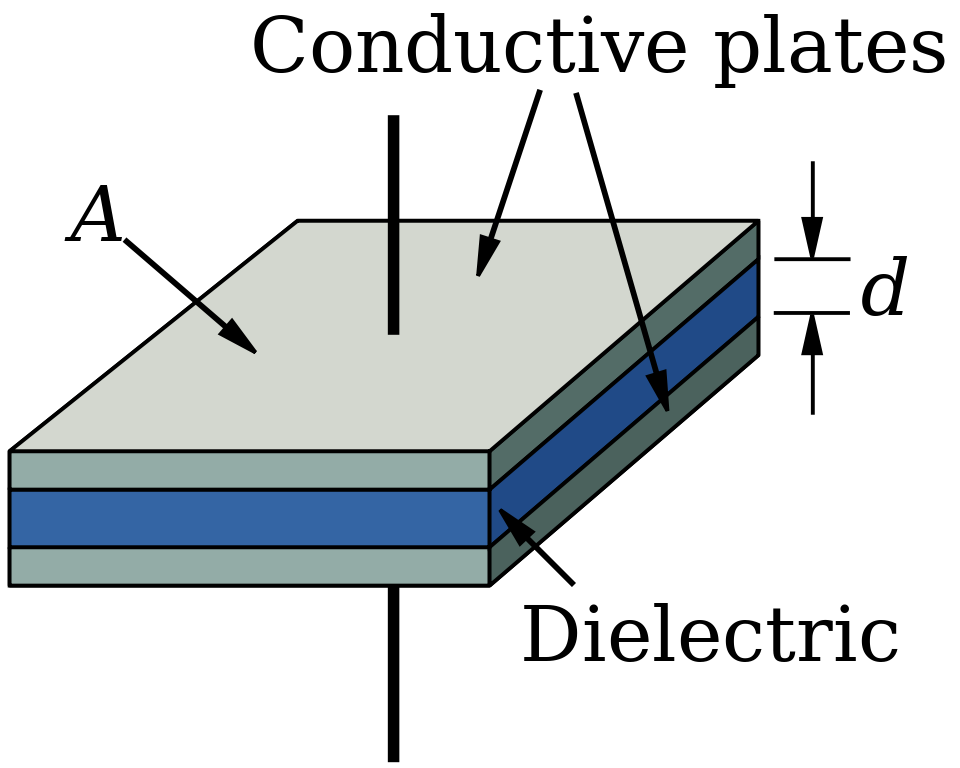
\includegraphics[scale = 0.125]{Images/Elektriciteit/Condensator.png}
    \end{center}
    
    \noindent De \textbf{capaciteit} (Farad) van een condensator is de \textbf{absolute waarde} van de verhouding tussen de elektrische lading ($ Q $) op een van de geleiders en het potentiaalverschil tussen de twee geleiders.
    
    \begin{equation*}
        C = |\dfrac{Q}{\Delta V}|
    \end{equation*}
\end{theo}

\begin{app}[Parallelle plaatcondensator]{Parallelle plaatcondensator}

    \begin{minipage}{.76\textwidth} 
        Elke geleidende plaat heeft een oppervlakte $A$ en ze zijn gescheiden door een afstand $d$. We nemen aan dat $d$ klein is tegenover de afmetingen van de platen en dus dat het elektrisch veld $\Vec{E}$ uniform is tussen de platen.
        Het elektrische veld, zoals we weten, tussen twee nabije, parallelle platen heeft grootte: $E = \tfrac{\sigma}{\epsilon_0}$ en zijn richting is loodrecht op de platen.
        Sinds $\sigma$ lading per oppervlakte is, bekomen we:
        \begin{equation*}
            E = \dfrac{Q}{\epsilon_0A}
        \end{equation*}
        We weten ook het verband tussen het elektrisch veld en het potentiaal, namelijk:
        \begin{equation*}
            \Delta V = - \int_{a}^{b} \Vec{E} \cdot d\Vec{\ell}
        \end{equation*}
        We berekenen nu op een antiparallel pad:
        \begin{equation*}
             \Delta V = - \int_{a}^{b} Ed\ell\cos(\pi) = \int_{a}^{b} Ed\ell = \dfrac{Q}{\epsilon_0A}\int_{a}^{b}d\ell = \dfrac{Qd}{\epsilon_0A}
        \end{equation*}
        We kunnen nu de capaciteit hieruit bepalen:
        \begin{equation*}
            C = \dfrac{Q}{\Delta V} = \epsilon_0\dfrac{A}{d}
        \end{equation*}
    \end{minipage}
    \begin{minipage}{.2\textwidth}
        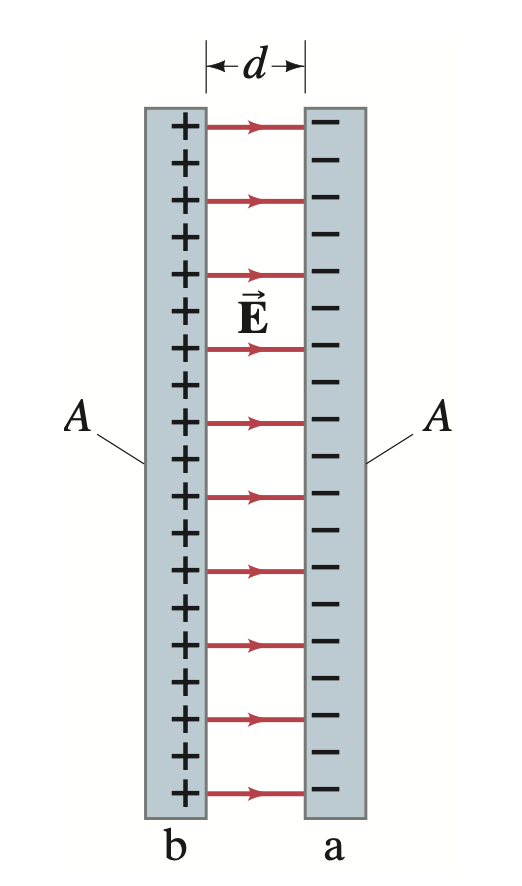
\includegraphics[scale = 0.43]{Images/Elektriciteit/ParallellePlatenCapaciteit.png}
    \end{minipage}
    
\end{app}

% \begin{ex}[Cylindrische condensator]{Cylindrische condensator}
%     \centering
%     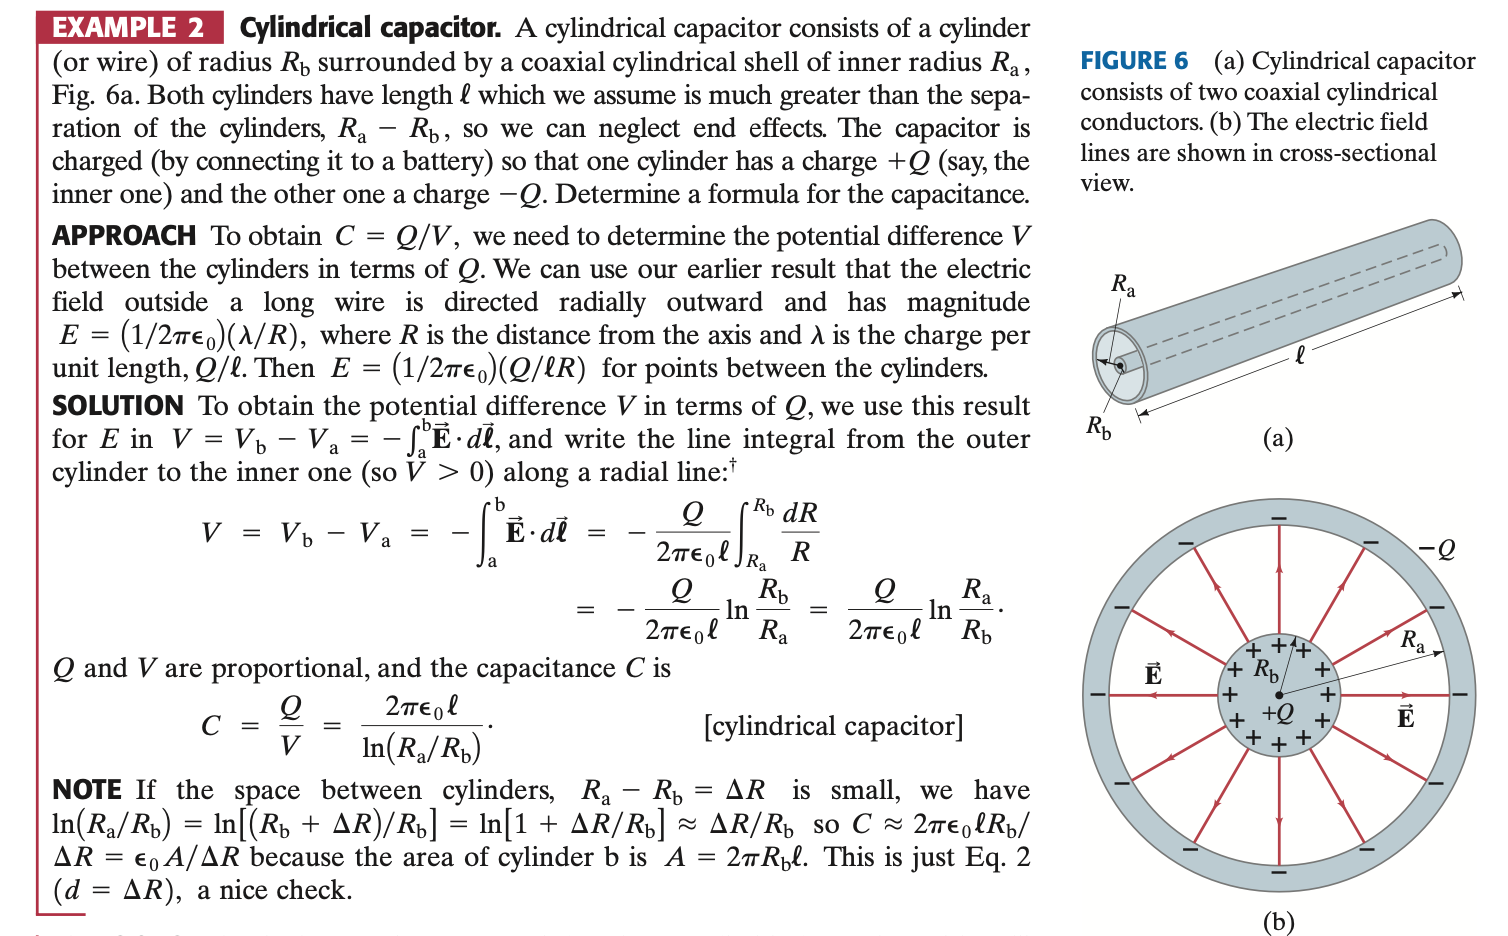
\includegraphics[scale = 0.55]{Examples/Elektriciteit/CyllindrischeCondensator.png}
% \end{ex}

% \begin{ex}[Sferische condensator]{Sferische condensator}
%     \centering
%     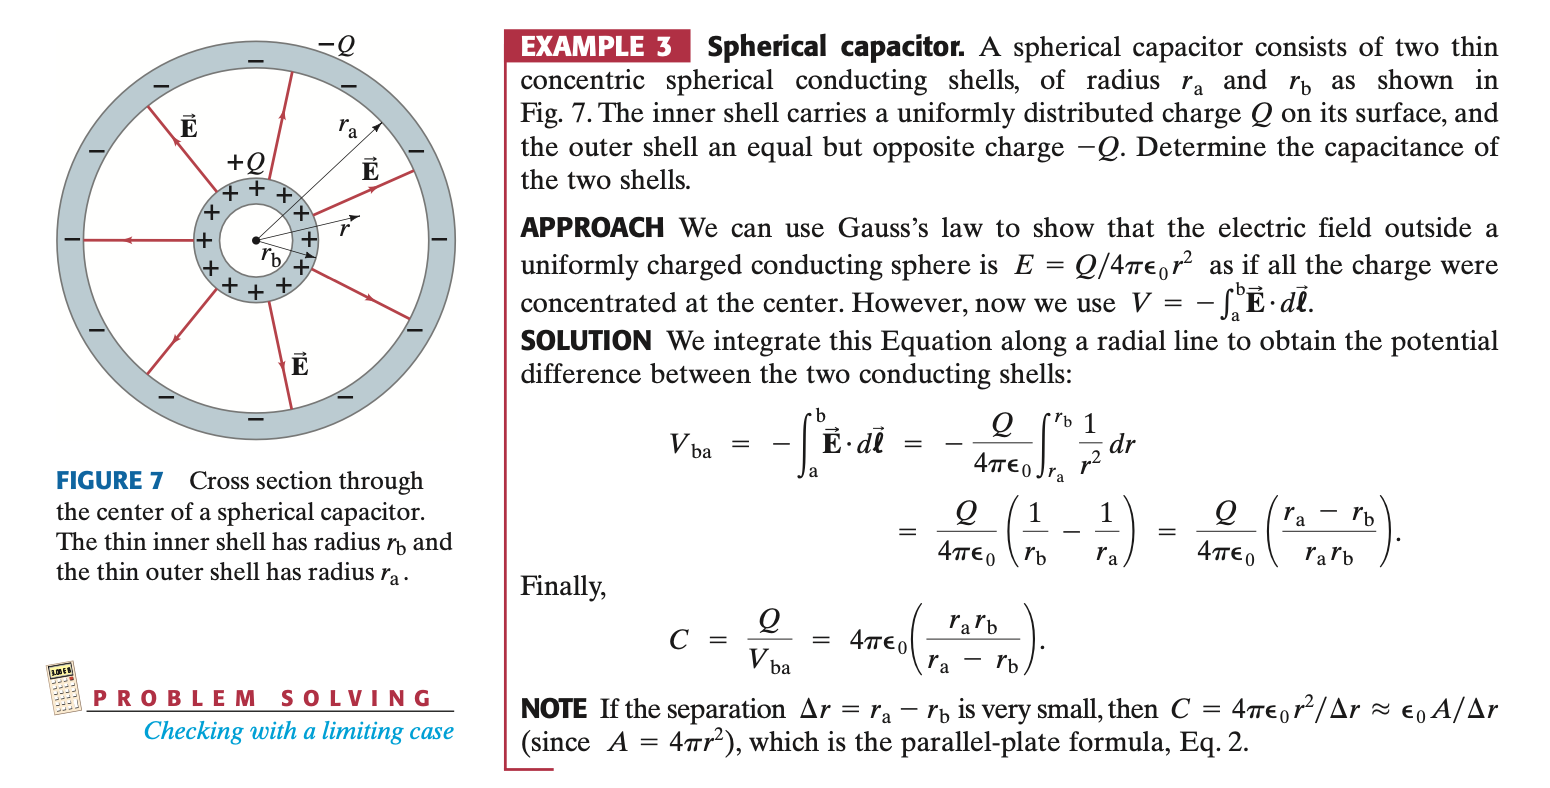
\includegraphics[scale = 0.55]{Examples/Elektriciteit/SferischeCondensator.png}
% \end{ex}

\newpage

\begin{theo}[Parallellschakeling]{Parallellschakeling}
    Een \textbf{parallelschakeling} is een configuratie van condensatoren waarbij de stroom over de individuele condensatoren wordt verdeeld en de spanning op alle condensatoren gelijk is. 
    \begin{center}
        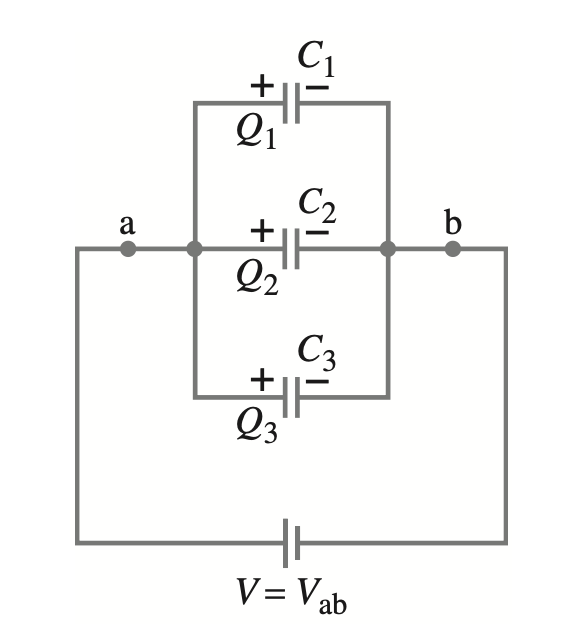
\includegraphics[scale = 0.35]{Images/Elektriciteit/Parallelleschakeling.png}
    \end{center}
\end{theo}

\begin{pro}[Eigenschappen van een parallellschakeling]{pro - Parallellschakeling}
    \begin{itemize}
        \item $\Delta V = \Delta V_i$
        \item $Q = \sum_i Q_i$
        \item $C_{eq} = \sum_i C_i $
    \end{itemize}
\end{pro}

\begin{theo}[Serieschakeling]{Serieschakeling}
    Een \textbf{serieschakeling} is een configuratie van condensatoren waarbij de stroom door de individuele condensatoren gelijk is en de spanning over alle condensatoren wordt verdeeld. 
    \begin{center}
        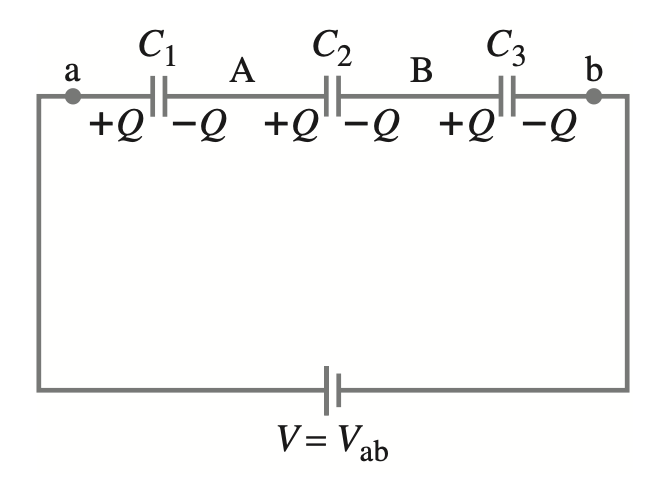
\includegraphics[scale = 0.35]{Images/Elektriciteit/Serieschakeling.png}
    \end{center}
\end{theo}

\begin{pro}[Eigenschappen van een serieschakeling]{pro - Serieschakeling}
    \begin{itemize}
        \item $\Delta V = \sum_i \Delta V_i$
        \item $Q = Q_i$
        \item $\dfrac{1}{C_{eq}} = \sum_i\dfrac{1}{C_i}$
    \end{itemize}
\end{pro}

\newpage

% \begin{ex}[Voorbeeld: Herkoppelen van geladen condensatoren]{Herkoppelen van geladen condensatoren}
%     \centering
%     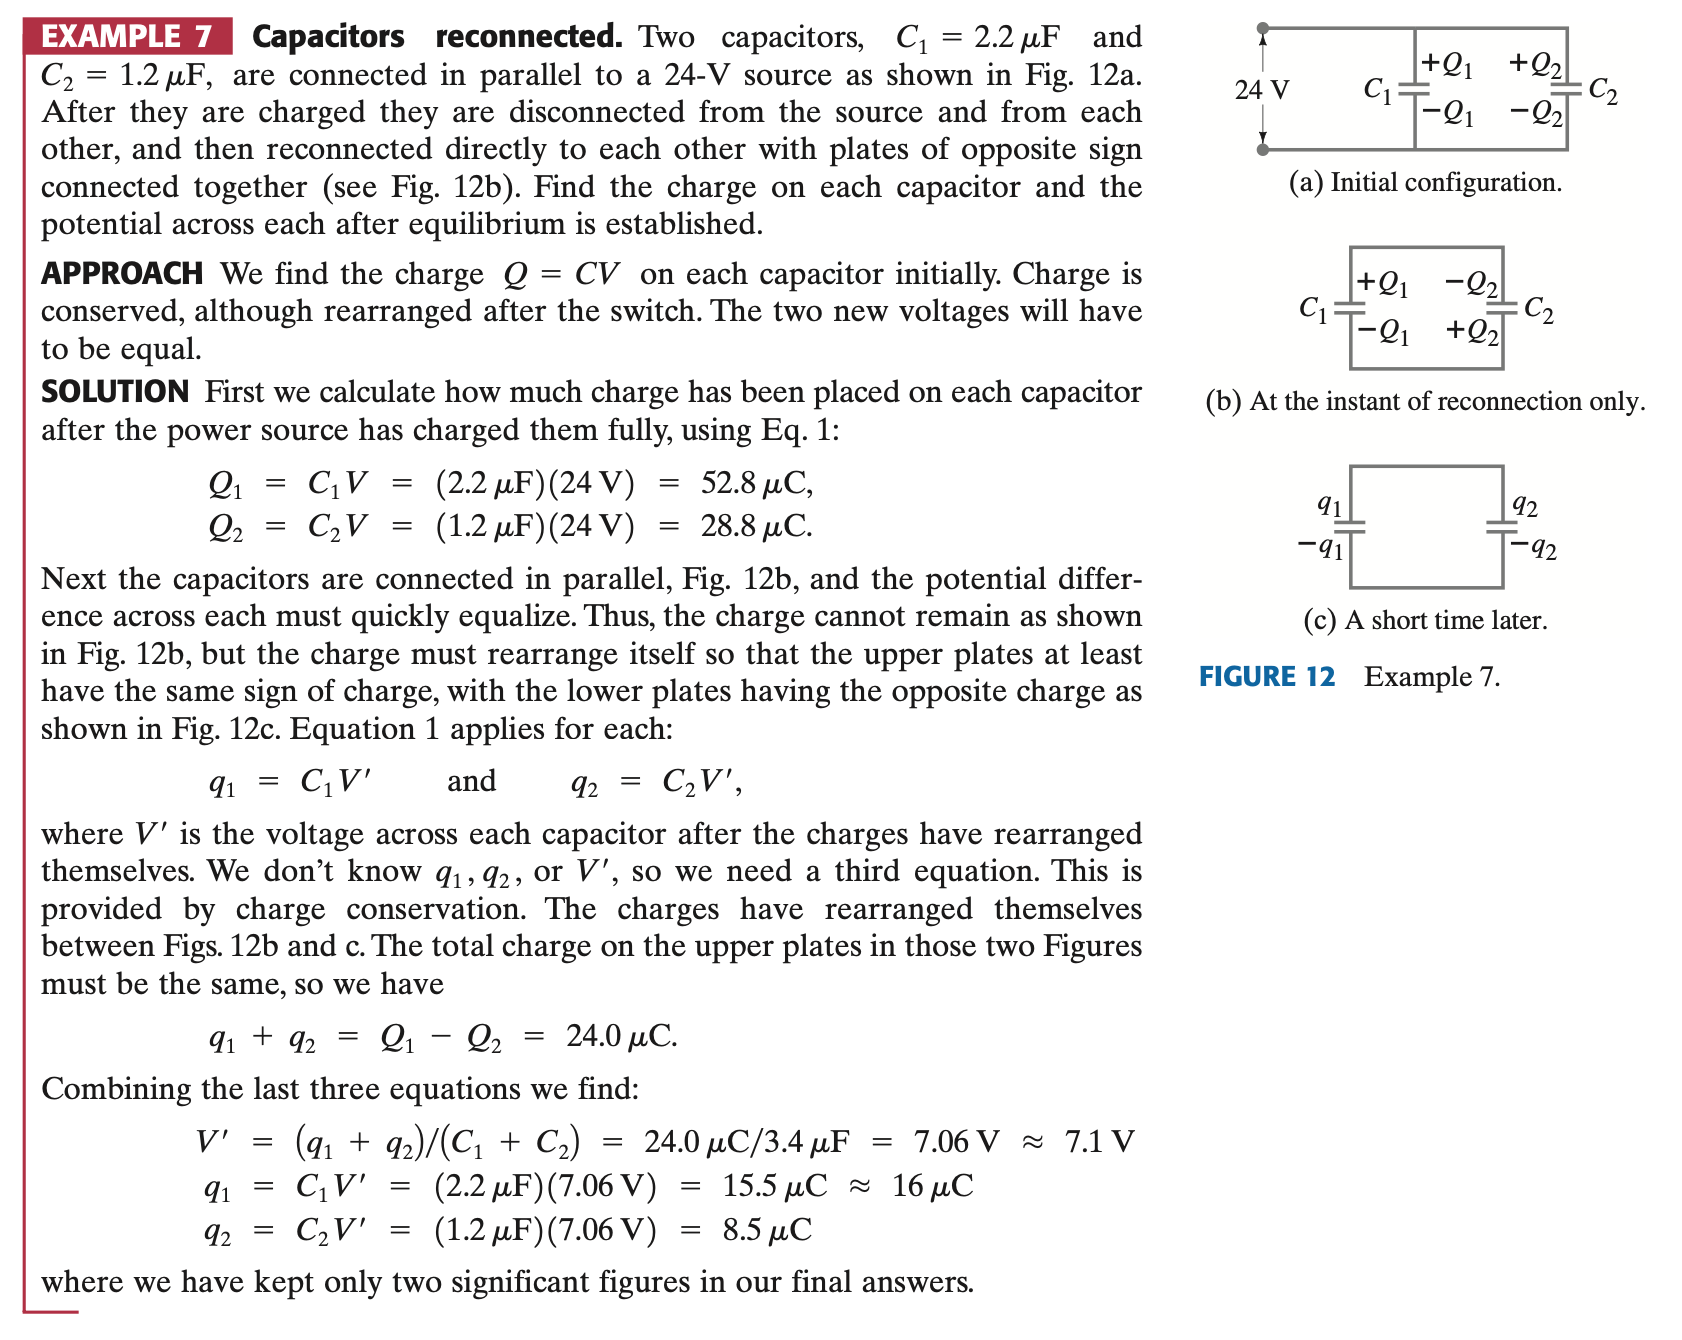
\includegraphics[scale = 0.52]{Examples/Elektriciteit/GeladenCondensatorenHerkoppelen.png}
% \end{ex}

\begin{theo}[Elektrische energie opslag]{Elektrische energie opslag}

    De opgeslagen energie in een condensator is gelijk aan de arbeid dat is verricht om hem op te laden.
    
    % Het netto-effect van het opladen van een condensator is dat de lading van de ene plaat wordt verwijderd en aan de andere plaat wordt toegevoegd. Dit is wat een batterij doet als hij op een condensator wordt aangesloten. 
    
    Een condensator wordt niet onmiddellijk opgeladen. Daar is tijd voor nodig. Aanvankelijk, als de condensator ongeladen is, is er geen arbeid nodig om het eerste beetje lading over te brengen. 
    
    % Wanneer er wat lading op elke plaat is, moet er door de elektrische afstoting meer lading van hetzelfde teken worden toegevoegd. 
    
    Hoe meer lading er al op een plaat zit, hoe meer arbeid er nodig is om extra lading toe te voegen. De arbeid die nodig is om een kleine hoeveelheid lading $dq$ toe te voegen, wanneer een potentiaalverschil $\Delta V$ over de platen loopt, is $dW = \Delta V dq$. Aangezien $\Delta V = \dfrac{Q}{C}$ op elk moment, is de arbeid die nodig is om een totale lading Q op te slaan
    \begin{equation*}
        W = \int_0^Q \Delta V dq = \dfrac{1}{C} \int_0^Q qdq = \dfrac{1}{2}\dfrac{Q^2}{C}
    \end{equation*}
    Dus we kunnen zeggen dat de opgeslagen energie 
    \begin{equation*}
        U = \dfrac{1}{2}\dfrac{Q^2}{C} = \dfrac{1}{2}C(\Delta V)^2 = \dfrac{1}{2}Q\Delta V
    \end{equation*}
    is wanneer de condensator ladingen $+Q$ en $-Q$ bezit op zijn platen.
    \begin{center}
        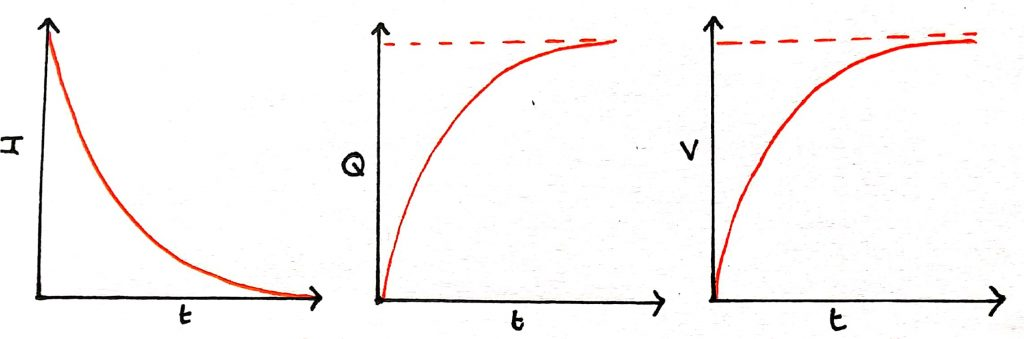
\includegraphics[scale = 0.25]{Images/Elektriciteit/OpladenGrafieken.jpg}
    \end{center} 
    \noindent De \textbf{energiedichtheid} van een condensator wordt gegeven door de volgende formule:

    \begin{equation*}
        U_E = \dfrac{1}{2}\epsilon_0E^2
    \end{equation*}
\end{theo}

\begin{theo}[Condensatoren met een diëlektricum]{Condensatoren met een diëlektricum}
    % In de meeste condensatoren bevindt zich tussen de platen een \textbf{isolerende} materiaal, zoals papier of plastic, dat een \textbf{diëlektricum} wordt genoemd. Dit heeft meerdere nutten. Ten eerste breken diëlektrische materialen minder snel af dan lucht, zodat hogere spanningen kunnen worden toegepast zonder dat lading over de spleet gaat. Verder maakt een diëlektricum het mogelijk de platen dichter bij elkaar te plaatsen zonder elkaar te raken, waardoor de capaciteit toeneemt omdat afstand kleiner is. Tenslotte is experimenteel 
    
    We kunnen in de plaats van vacuüm ook andere diëlectrica (isolator) tussen de platen steken. Er is vastgesteld dat als het diëlektricum de ruimte tussen de twee geleiders vult, de capaciteit toeneemt met een factor $K$, die bekend staat als de \textbf{diëlektrische constante}. Er geldt dus
    \begin{equation*}
        C = KC_0
    \end{equation*}
    waarbij $C_0$ de capaciteit is waarbij de ruimte in de condensator vacuüm is.\\

    \noindent Bij parallelle platen wordt deze formule dan:
    \begin{equation*}
        C = K\epsilon_0\dfrac{A}{d} = \epsilon\dfrac{A}{d}
    \end{equation*}
    \vspace{-0.5cm}
\end{theo}

\newpage

\begin{app}[Moleculaire beschrijving van diëlektrica]{Moleculaire beschrijving van diëlektrica}
    \vspace{-0.5cm}
    \begin{minipage}{.75\textwidth}
        Als we beginnen van een geïsoleerde situatie, zie figuur (a), dan kunnen we de capaciteit met de volgende formule beschrijven
        \begin{equation*}
            C_0 = \dfrac{Q}{(\Delta V)_0}
        \end{equation*}
        \noindent waarbij het subscript $0$ voor vacuüm dient. Als we nu een diëlektricum toevoegen aan de constructie, dan zal door het elektrische veld de molecules van het diëlektricum zoals op figuur (b). Het effect van deze ordening is dat er nu een netto postieve en negatieve lading is op de uiteinde van het diëelektricum, zie figuur (c). Sommige van de elekrische veldlijen worden ook opgenomen door het diëlektricum, dus het elektrisch veld wordt verkleind. Het elektrisch veld in het diëlektricum $E_D$ kan gezien worden als het veld door de vrije ladingen van de platen en het veld van de geïnduceerde ladingen, zie figuur (d). De vectoriële som is dan
        \begin{equation*}
            \Vec{E}_D = \Vec{E}_0 + \Vec{E}_{ind}
        \end{equation*}
        ofwel
        \begin{equation*}
            E_D = E_0 - E_{ind} = \dfrac{E_0}{K}
        \end{equation*}
        Het geïnduceerd veld wordt dus berekend op de volgende manier:
        \begin{equation*}
            E_{ind} = E_0(1-\dfrac{1}{K})
        \end{equation*}
    \end{minipage}
    \hspace{0.5cm}
    \begin{minipage}{.18\textwidth}
        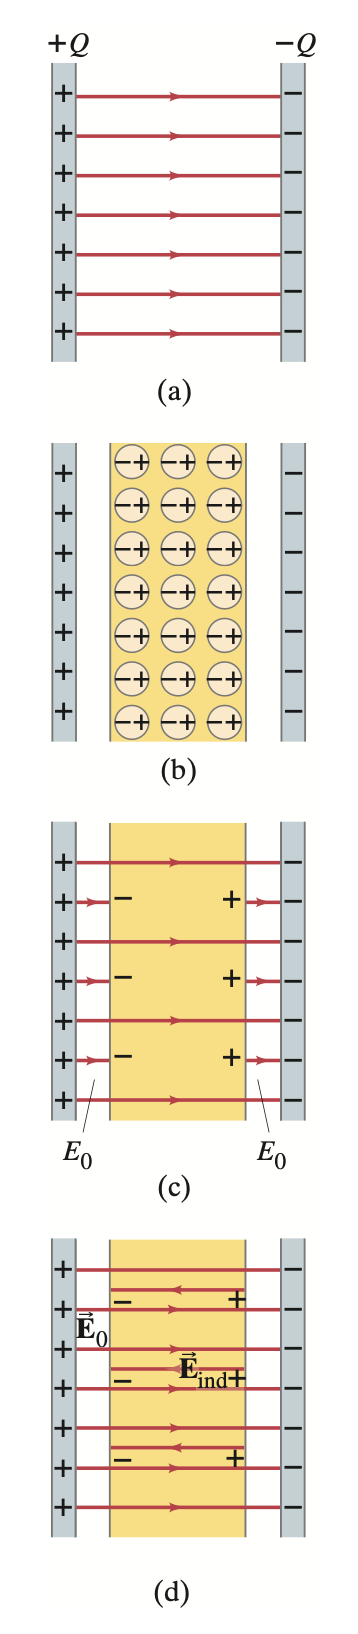
\includegraphics[scale = 0.4]{Images/Elektriciteit/MoleculaireBeschrijvingVanDielektrica.png}
    \end{minipage}
\end{app}

\begin{app}[Parallelle plaatcondensator met een diëlektricum]{Parallelle plaatcondensator met een diëlektricum}
    We hebben in de voorgaande hoofdstukken al de volgende formule besproken
    \begin{equation*}
        E_0 = \dfrac{\sigma}{\epsilon_0}
    \end{equation*}
    waarbij $\sigma$ de oppervlakte ladingsdichtheid is op de geleider. Deze lading $Q$ wordt vaak de vrije lading genoemd.
    Als we nu het geïnduceerde veld bekijken, dan krijgen we:
    \begin{equation*}
        E_{ind} = \dfrac{\sigma_{ind}}{\epsilon_0}
    \end{equation*}
    Hier is $\sigma_{ind}$ de oppervlakte ladingsdichtheid op de isolator. De lading $Q_{ind}$ wordt vaak de gebonden lading genoemd. Uit deze laatste twee formules kunen we de volgende nuttige resultaten bekomen:
    \begin{equation*}
            \sigma_{ind} = \sigma(1-\dfrac{1}{K}), \qquad Q_{ind} = Q(1-\dfrac{1}{K})
    \end{equation*}
\end{app}



